\setcounter{chapter}{2}
\renewcommand{\thetheorem}{3.\arabic{theorem}}
\setcounter{theorem}{0}

\chapter{Set Theory}

In this chapter, we formalize the language of sets, which provides the universal framework for all modern mathematical structures, including the vector spaces we will investigate later.

\subsection{Basic Definitions and Notation}

\begin{definition}[Set]
A \qt{set} is a collection of distinct objects, which are referred to as the \textit{elements} of the set.
\end{definition}

In our notation, we denote sets typically by capital letters. If an object $x$ is an element of a set $M$, we write $x \in M$. If it is not, we write $x \notin M$.

\begin{remark}
Crucially, within a set, the order of elements is irrelevant, and repetitions do not contribute to the set's identity. For example:
\[
M = \{1, 3, \text{moon}\} = \{3, \text{moon}, 1\}
\]
\[
M = \{1, 1, 1\} = \{1\}
\]
\end{remark}

We frequently define sets using a property or condition $A(x)$ that the elements must satisfy. The standard notation for this \qt{set-builder} form is:
\[
M = \{x \mid A(x)\} \quad \text{or} \quad M = \{x : A(x)\}
\]

\begin{example}[Set-Builder Notation]
The set of integers whose square is less than or equal to $9$ is written as:
\[
\{x \in \mathbb{Z} \mid x^2 \le 9\} = \{-3, -2, -1, 0, 1, 2, 3\}
\]
\end{example}

\begin{definition}[The Empty Set]
The \qt{empty set}, denoted by $\emptyset$ or $\{\}$, is the unique set containing no elements.
\end{definition}

It is important to note that a set is allowed to contain another set as one of its elements. For instance, consider the set $M = \{1, \text{elephant}, \{a, 5\}\}$. Here, the set $\{a, 5\}$ is a single element of $M$. Similarly, we can define a set containing only the empty set: $M = \{\emptyset\}$, which is a set containing exactly one element.

\subsection{Subsets and Inclusion}

We now define how sets relate to one another in terms of containment.

\begin{definition}[Subset and Proper Subset]
Let $P$ and $Q$ be sets.
\begin{enumerate}
    \item We say $P$ is a \qt{subset} of $Q$, denoted $P \subseteq Q$, if every element of $P$ is also an element of $Q$. Formally: $\forall x \in P : x \in Q$.
    \item We say $P$ is a \qt{proper subset} of $Q$, denoted $P \subsetneq Q$, if $P \subseteq Q$ and $P \ne Q$. 
    \item We write $P \not\subseteq Q$ to denote that $P$ is not a subset of $Q$, meaning $\neg(P \subseteq Q)$.
\end{enumerate}
\end{definition}

\begin{remark}
Note that some authors use $P \subset Q$ to denote proper subsets, while others use it for generic subsets.
\end{remark}

\begin{claim*}
For any set $Q$, the empty set is a subset of $Q$ (i.e., $\emptyset \subseteq Q$).
\end{claim*}

\subsection{Set Operations}

Just as we have logical operators for statements, we have operations to combine or modify sets. Let $A$ and $B$ be subsets of a universal set $X$.

\begin{enumerate}
    \item \textbf{Intersection:} $A \cap B = \{x \in X \mid x \in A \wedge x \in B\}$.
    \item \textbf{Union:} $A \cup B = \{x \in X \mid x \in A \vee x \in B\}$.
    \item \textbf{Difference:} $A \setminus B = \{x \in X \mid x \in A \wedge x \notin B\}$.
    \item \textbf{Complement:} The complement of $A$ in $X$ is $A^c = X \setminus A = \{x \in X \mid x \notin A\}$.
\end{enumerate}

\begin{center}
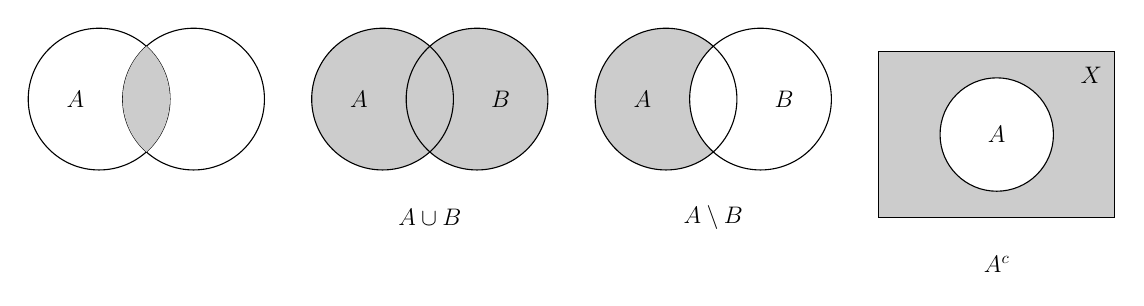
\begin{tikzpicture}[scale=0.6, every node/.style={transform shape}]
    % Intersection
    \begin{scope}[shift={(0,0)}]
        \draw (0,0) circle (1.5cm);
        \draw (2,0) circle (1.5cm);
        \clip (0,0) circle (1.5cm);
        \fill[gray!40] (2,0) circle (1.5cm);
        \node at (-0.5,0) {\Large $A$};
        \node at (2.5,0) {\Large $B$};
        \node at (1,-2.5) {\Large $A \cap B$};
    \end{scope}

    % Union
    \begin{scope}[shift={(6,0)}]
        \fill[gray!40] (0,0) circle (1.5cm);
        \fill[gray!40] (2,0) circle (1.5cm);
        \draw (0,0) circle (1.5cm);
        \draw (2,0) circle (1.5cm);
        \node at (-0.5,0) {\Large $A$};
        \node at (2.5,0) {\Large $B$};
        \node at (1,-2.5) {\Large $A \cup B$};
    \end{scope}

    % Difference
    \begin{scope}[shift={(12,0)}]
        \fill[gray!40] (0,0) circle (1.5cm);
        \begin{scope}
            \clip (2,0) circle (1.5cm);
            \fill[white] (0,0) circle (1.5cm);
        \end{scope}
        \draw (0,0) circle (1.5cm);
        \draw (2,0) circle (1.5cm);
        \node at (-0.5,0) {\Large $A$};
        \node at (2.5,0) {\Large $B$};
        \node at (1,-2.5) {\Large $A \setminus B$};
    \end{scope}
    
    % Complement
    \begin{scope}[shift={(18,-1.5)}]
        \fill[gray!40] (-1.5,-1) rectangle (3.5,2.5);
        \fill[white] (1,0.75) circle (1.2cm);
        \draw (-1.5,-1) rectangle (3.5,2.5);
        \draw (1,0.75) circle (1.2cm);
        \node at (1,0.75) {\Large $A$};
        \node at (3,2) {\Large $X$};
        \node at (1,-2) {\Large $A^c$};
    \end{scope}
\end{tikzpicture}
\end{center}

\subsection{Cartesian Products}

To handle ordered pairs and higher-dimensional structures, we introduce the Cartesian product.

\begin{definition}[Cartesian Product]
The \qt{Cartesian product} of two sets $X$ and $Y$ is the set of all ordered pairs $(x, y)$ where $x \in X$ and $y \in Y$:
\[
X \times Y = \{(x, y) \mid x \in X, y \in Y\}
\]
\end{definition}

This construction generalizes to $n$ sets. We denote the $n$-fold product of a set $X$ with itself as $X^n$:
\[
X^n = \underbrace{X \times \dots \times X}_{n \text{ times}} = \{(x_1, \dots, x_n) \mid x_i \in X \text{ for } 1 \le i \le n\}
\]
The elements of $X^n$ are called $n$-tuples. For example, $X^2 = X \times X$, and $X^3 = X \times X \times X = \{(x_1, x_2, x_3) \mid x_1, x_2, x_3 \in X\}$, and so forth.

\begin{example}[Cartesian Products in the Plane]
If $X = \mathbb{R}$, then $X^2 = \mathbb{R} \times \mathbb{R} = \mathbb{R}^2$ represents the standard Euclidean plane. If we take $X = [0, 2]$ and $Y = [1, 2]$, then $X \times Y$ represents a rectangle in the plane with corners at $(0,1), (2,1), (0,2),$ and $(2,2)$.

\begin{center}
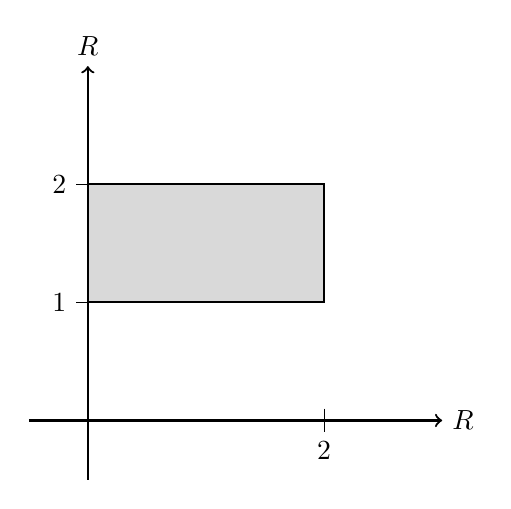
\begin{tikzpicture}[scale=1.5]
    % Axes
    \draw[->, thick] (-0.5, 0) -- (3, 0) node[right] {$\mathbb{R}$};
    \draw[->, thick] (0, -0.5) -- (0, 3) node[above] {$\mathbb{R}$};
    
    % Rectangle X \times Y
    \fill[gray!30] (0, 1) rectangle (2, 2);
    \draw[thick] (0, 1) rectangle (2, 2);
    
    % Ticks and Labels
    \draw (2, 0.1) -- (2, -0.1) node[below] {$2$};
    \draw (0.1, 1) -- (-0.1, 1) node[left] {$1$};
    \draw (0.1, 2) -- (-0.1, 2) node[left] {$2$};
\end{tikzpicture}
\end{center}
\end{example}

\subsection{Power Sets and Cardinality}

\begin{definition}[Power Set]
Let $X$ be a set. The \qt{power set} of $X$, denoted by $\mathcal{P}(X)$ or $2^X$, is the set of all subsets of $X$:
\[
\mathcal{P}(X) = \{Q \mid Q \subseteq X\}
\]
\end{definition}

\begin{example}[Power Set of a Finite Set]
For $X = \{1, 2, 3\}$, the power set is:
\[
\mathcal{P}(X) = \{\emptyset, \{1\}, \{2\}, \{3\}, \{1, 2\}, \{1, 3\}, \{2, 3\}, \{1, 2, 3\}\}
\]
Note that $\mathcal{P}(X)$ contains $8$ elements.
\end{example}

\begin{definition}[Cardinality]
If $X$ is a finite set, meaning a set with finitely many elements $X = \{x_1, \dots, x_n\}$, we say that the \qt{cardinality} of $X$ is the number of elements in $X$, denoted by $|X| = n$ or $\text{card}(X) = n$.
\end{definition}

\begin{exercise}
Let $A$ be a finite set. Prove by induction that the cardinality of its power set is given by:
\[
|\mathcal{P}(A)| = 2^{|A|}
\]
\end{exercise}

\subsection{A Note on the Foundations: Russell's Paradox}

In the early development of set theory, it was assumed that any property $A(x)$ could define a set (Naive Set Theory). However, Bertrand Russell showed that this leads to a contradiction.

Suppose there exists a \qt{set of all sets}, denoted by $S$. We then define a subset $R \subseteq S$ as follows:
\[
R := \{X \in S \mid X \notin X\}
\]
Now, we ask: is $R$ an element of itself?
\begin{itemize}
    \item If $R \in R$, then by the definition of $R$, it must be that $R \notin R$. This is a contradiction.
    \item If $R \notin R$, then by the definition of $R$, it must be that $R \in R$. This is also a contradiction.
\end{itemize}

\begin{claim*}
$S$ is not a set.
\end{claim*}

This paradox led to the development of Axiomatic Set Theory (e.g., Zermelo-Fraenkel), which places specific restrictions on how sets can be constructed to ensure mathematical consistency.
